% =====================================================================
% Supplementary Information - Digital phenotyping of mental disorders (NHB)
% Compile: pdflatex supplementary_information_NHB.tex (twice). Figures in ./figures/
% Contains: Supplementary Methods, Supplementary Tables 1--4, Supplementary Figures 1--3.
% Extended Data figures are provided separately in extended_data_NHB.tex.
% =====================================================================
\documentclass[11pt]{article}
\usepackage[margin=1in]{geometry}
\usepackage[T1]{fontenc}
\usepackage[utf8]{inputenc}
\usepackage{mathptmx}
\usepackage{graphicx}
\usepackage{booktabs}
\usepackage{amsmath,amssymb}
\usepackage{color}
\usepackage{caption}
\DeclareCaptionLabelSeparator{pipe}{\ \textbar\ }
\captionsetup[figure]{name=Supplementary Fig., labelsep=pipe, font=small, labelfont=bf,
  singlelinecheck=false, justification=raggedright, skip=3pt}
\captionsetup[table]{name=Supplementary Table, labelsep=pipe, font=small, labelfont=bf,
  singlelinecheck=false, justification=raggedright, skip=3pt}
\usepackage{longtable}
\usepackage[colorlinks=true,urlcolor=blue,citecolor=blue]{hyperref}

\begin{document}

\begin{center}
{\LARGE\bfseries Supplementary Information}\\[6pt]
{\large Robust but scale-dependent digital phenotypes of mental disorders in 128{,}000 Reddit
users}
\end{center}

\vspace{0.6em}
\noindent This Supplementary Information contains Supplementary Methods, Supplementary
Tables~1--4 and Supplementary Figures~1--3. Extended Data Figures~1--10 are provided
separately. All items are cited from the main text.

\tableofcontents

\section*{Supplementary Methods}
\addcontentsline{toc}{section}{Supplementary Methods}

\paragraph*{Provenance and cohort construction.}
Reddit comments and submissions (2006--2023) were assembled from a public Pushshift snapshot and
processed in five stages (Table~\ref{tab:st3}): raw dump; Phase-1 case identification by a
first-person self-reported-diagnosis grammar; Phase-2 full-history extraction (4{,}950{,}144
posts); bot and quality filtering (4{,}771{,}571 posts); shadow-$t_0$ assignment (3{,}730{,}213
users); and propensity-score matching (723{,}574 users; 128{,}003 diagnosed, 595{,}571
comparison). Each stage is scripted and logged; the raw user-level data are not redistributed.

\paragraph*{Self-reported-diagnosis grammar (silver standard).}
Cases were defined by inclusion patterns of the form
\texttt{I (was|have been|am|got) (officially|clinically|formally|professionally)? diagnosed with
[\ldots]}, with exclusion of third-party, negated and self-diagnosed statements, and a
\texttt{spaCy} dependency gate requiring the lemma \texttt{diagnose} as a verb with a
first-person subject or object and no negation. Retrospective time expressions were flagged but
not rejected. The resulting label is a \emph{self-reported diagnosis} (behavioural proxy), not a
clinical record.

\paragraph*{Propensity-score matching and balance.}
Matching used a 1:5 ratio without replacement within exact tenure quartiles, an 11-feature
propensity model and a caliper of 0.2 standard deviations; inverse-probability weighting and
entropy balancing are reported as sensitivity. Maximum standardised mean difference fell from
0.054 to 0.0097, with an effective sample size of 586{,}010 after weighting.

\paragraph*{Feature engineering.}
101 candidate features in 14 dimensions (linguistic, affective, cognitive,
behavioural, temporal, social) were computed per user; sentiment and emotion-lexicon features
used VADER. Three features were dropped for zero training interquartile range and five features
circular with case identification (subreddit entropy and Herfindahl, primary- and
mental-health-subreddit ratios) were excluded, leaving 93 analysis features (930 tests).
Features were winsorised to [0.5, 99.5] percentiles and robust-scaled on training splits only.
The dimension inventory and the effect-size distribution are in Table~\ref{tab:st1}.

\paragraph*{Statistics, multiplicity and seeds.}
Hedges' $g$ with Welch $P$ values and Benjamini--Hochberg false-discovery-rate control was used
throughout; time-series associations used first differences, detrending, Newey--West standard
errors and block-permutation tests where independence was not assumed. Pre-specified seeds were
42 (analysis) and 2025 (trajectory, mixture, placebo); placebo difference-in-differences used
100 draws with the pseudo-$t_0$ shifted 90--360 days (random sign). All reported numbers trace
to a stored result file.

\paragraph*{External data and ecological caution.}
National suicide mortality was taken from CDC underlying-cause-of-death data (ICD-10 X60--X84,
age-adjusted per 100{,}000; 2008--2022 overlap) and major-depressive-episode prevalence from
SAMHSA NSDUH (2015--2022, with the 2021 methodological break noted). External populations are
national and are not equated with Reddit users; the associations are ecological.

\section*{Supplementary Tables}
\addcontentsline{toc}{section}{Supplementary Tables}

\begin{table}[h]\centering\small
\caption{Cohort layers, feature set and effect-size distribution.}
\label{tab:st1}
\begin{tabular}{ll}
\toprule
Item & Value \\
\midrule
Matched layer L1 (case / comparison) & 128{,}003 / 595{,}571 \\
Feature layer L2 (case / comparison) & 127{,}168 / 594{,}817 \\
Trajectory layer L3 (case / comparison) & 123{,}986 / 565{,}598 \\
Case composition (L1) & ADHD 37{,}645; depression 30{,}645; anxiety 14{,}426; autism 10{,}225; \\
 & bipolar 10{,}007; PTSD 8{,}282; borderline 6{,}083; OCD 5{,}736; \\
 & schizophrenia 2{,}461; eating 1{,}688; unlabelled 805 \\
Two or more diagnoses & 39{,}059 (30.5\%); top pair anxiety--depression 15{,}140 \\
Analysis features (after removing 5 circular features) & 93 \\
Dimensions & 14 (linguistic, affective, cognitive, behavioural, temporal, social, \ldots) \\
Feature--disorder tests & 930 \\
FDR-significant (BH, global) & 765 (82.3\%) \\
Mean $|$Hedges' $g|$ & 0.21 \\
Median $|g|$ & 0.12 \\
IQR of $|g|$ & 0.04--0.27 \\
95th percentile of $|g|$ & 0.76 \\
Subsampling AUROC s.d. & $<$0.005 \\
Confound-adjusted correlation with primary estimates & $r=0.989$ \\
Single-disorder AUROC range & 0.84--0.92 \\
Leakage mean $|\Delta$AUROC$|$ (diagnosis posts excluded) & 0.006 \\
Dimension ablation (all / affective / temporal) & 0.886 / 0.825 / 0.597 \\
\bottomrule
\end{tabular}
\end{table}

\begin{table}[h]\centering\small
\caption{External validation robustness: behavioural volatility versus national suicide
mortality.}
\label{tab:st2}
\begin{tabular}{ll}
\toprule
Statistic & Value \\
\midrule
Raw Pearson $r$ & 0.906 \\
First-difference $r$ & 0.511 \\
Detrended $r$ & 0.473 \\
Permutation $p$ & $<$0.001 \\
Bootstrap 95\% CI & 0.77--0.97 \\
Leave-one-year-out range of $r$ & 0.03 \\
Posting intensity (detrended) & $-0.39$ \\
Language/severity composite & not significant after detrending \\
\bottomrule
\end{tabular}
\end{table}

\begin{table}[h]\centering\small
\caption{Reproducibility, provenance and assumptions.}
\label{tab:st3}
\begin{tabular}{ll}
\toprule
Item & Value \\
\midrule
Raw dump $\rightarrow$ Phase-1 candidates & reported in methods/provenance \\
Phase-2 full-history extraction & 4{,}950{,}144 posts \\
After bot/quality filtering & 4{,}771{,}571 \\
Shadow-$t_0$ assigned & 3{,}730{,}213 users \\
Matched layer (L1) & 128{,}003 / 595{,}571 \\
Feature layer (L2) & 127{,}168 / 594{,}817 \\
Trajectory layer (L3) & 123{,}986 / 565{,}598 \\
Maximum SMD (before / after IPTW) & 0.054 / 0.0097 \\
Effective sample size (IPTW) & 586{,}010 \\
Reliable windows (trajectory / calendar) & 17{,}451{,}019 / 17{,}247{,}283 \\
Identifier hashing & salted SHA-256; collision $\approx$0.1--0.2\% \\
Seeds (analysis / trajectory-mixture-placebo) & 42 / 2025 \\
Placebo draws (shift) & 100 (90--360 days, random sign) \\
MNAR silent windows (imputed) & 48.35\% (individual results use reliable windows) \\
External series & CDC suicide 2008--2022; NSDUH MDE 2015--2022 \\
\bottomrule
\end{tabular}
\end{table}

\begin{table}[h]\centering\small
\caption{Externally sourced clinical comorbidity pairs used for the primary Mantel test against
phenotypic dissimilarity (21 pairs, adjusted or pooled odds ratios). Sources are DOI-referenced;
see Supplementary References.}
\label{tab:st4}
\begin{tabular}{lllrl}
\toprule
Disorder A & Disorder B & OR & 95\% CI & Source \\
\midrule
depression & anxiety & 4.20 & 3.81--4.57 & Hasin 2018 (NESARC-III) \\
depression & OCD & 3.50 & 2.00--6.20 & Ruscio 2010 (NCS-R) \\
depression & PTSD & 4.40 & 3.92--5.03 & Hasin 2018 (NESARC-III) \\
depression & borderline & 5.20 & 4.70--5.74 & Hasin 2018 (NESARC-III) \\
depression & eating & 5.73 & 4.33--7.60 & Udo 2019 (NESARC-III) \\
depression & ADHD & 4.51 & 2.44--8.34 & Hartman 2023 (meta) \\
bipolar & OCD & 7.40 & 3.60--15.40 & Ruscio 2010 (NCS-R) \\
bipolar & schizophrenia & 6.90 & 1.20--41.40 & Kessler 2005 (NCS-R) \\
bipolar & ADHD & 8.72 & 5.47--13.89 & Hartman 2023 (meta) \\
bipolar & eating & 4.58 & 2.93--7.16 & Udo 2019 (NESARC-III) \\
anxiety & OCD & 7.60 & 3.40--16.90 & Ruscio 2010 (NCS-R) \\
anxiety & PTSD & 9.55 & 5.14--17.74 & Smith 2016 (NESARC-III) \\
anxiety & ADHD & 4.95 & 3.29--7.46 & Hartman 2023 (meta) \\
anxiety & eating & 6.21 & 4.77--8.06 & Udo 2019 (NESARC-III) \\
OCD & PTSD & 2.90 & 1.60--5.40 & Ruscio 2010 (NCS-R) \\
OCD & ADHD & 3.80 & 1.70--8.20 & Ruscio 2010 (NCS-R) \\
OCD & eating & 4.20 & 1.40--12.80 & Hudson 2007 (NCS-R) \\
PTSD & schizophrenia & 6.00 & 1.70--21.60 & Kessler 2005 (NCS-R) \\
PTSD & eating & 6.24 & 4.66--8.35 & Udo 2019 (NESARC-III) \\
borderline & eating & 7.75 & 5.83--10.31 & Udo 2019 (NESARC-III) \\
eating & ADHD & 3.10 & 1.50--6.20 & Hudson 2007 (NCS-R) \\
\bottomrule
\end{tabular}
\end{table}

\clearpage
\section*{Supplementary Figures}
\addcontentsline{toc}{section}{Supplementary Figures}

\begin{figure}[h]\centering
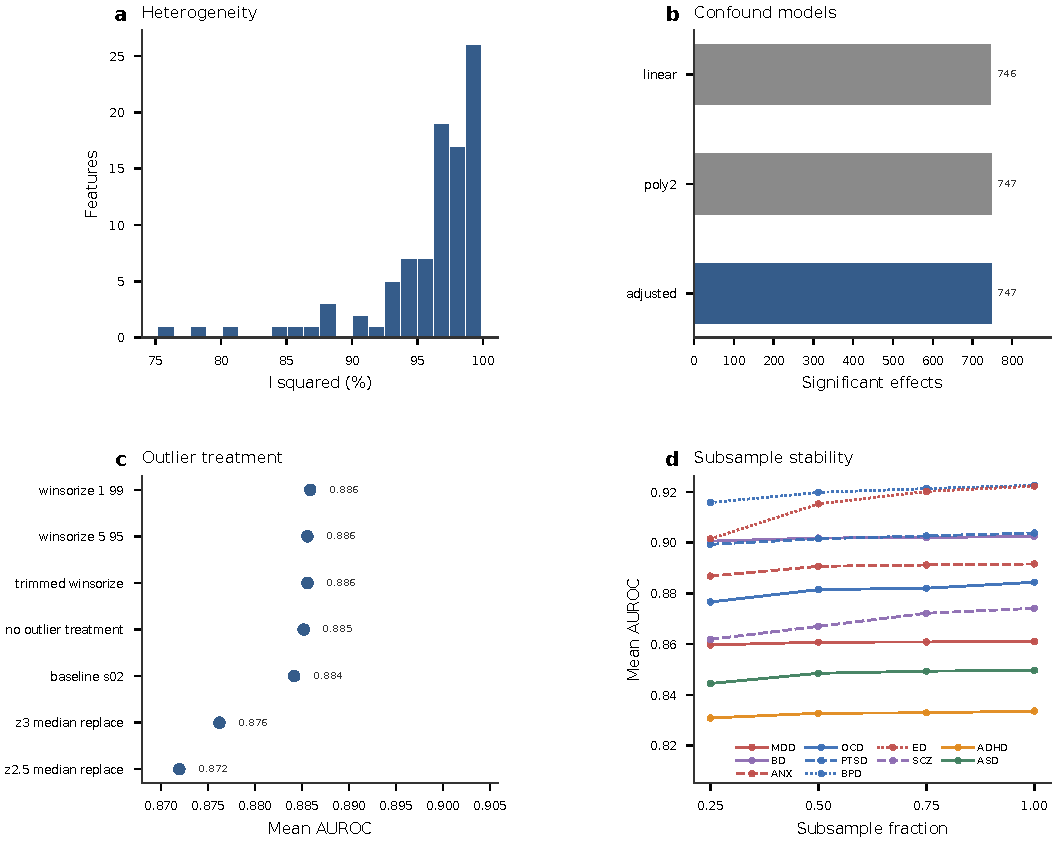
\includegraphics[width=0.98\linewidth]{figures/si1_sensitivity_suite_lyc.pdf}
\caption{\textbf{Sensitivity suite.} \textbf{a}, Distribution of between-disorder heterogeneity
($I^2$). \textbf{b}, Significant effects under linear, polynomial-2 and confound-adjusted
models. \textbf{c}, Mean AUROC under the outlier-treatment strategies. \textbf{d},
Subsample-size stability per disorder.}
\label{fig:s1}
\end{figure}

\begin{figure}[h]\centering
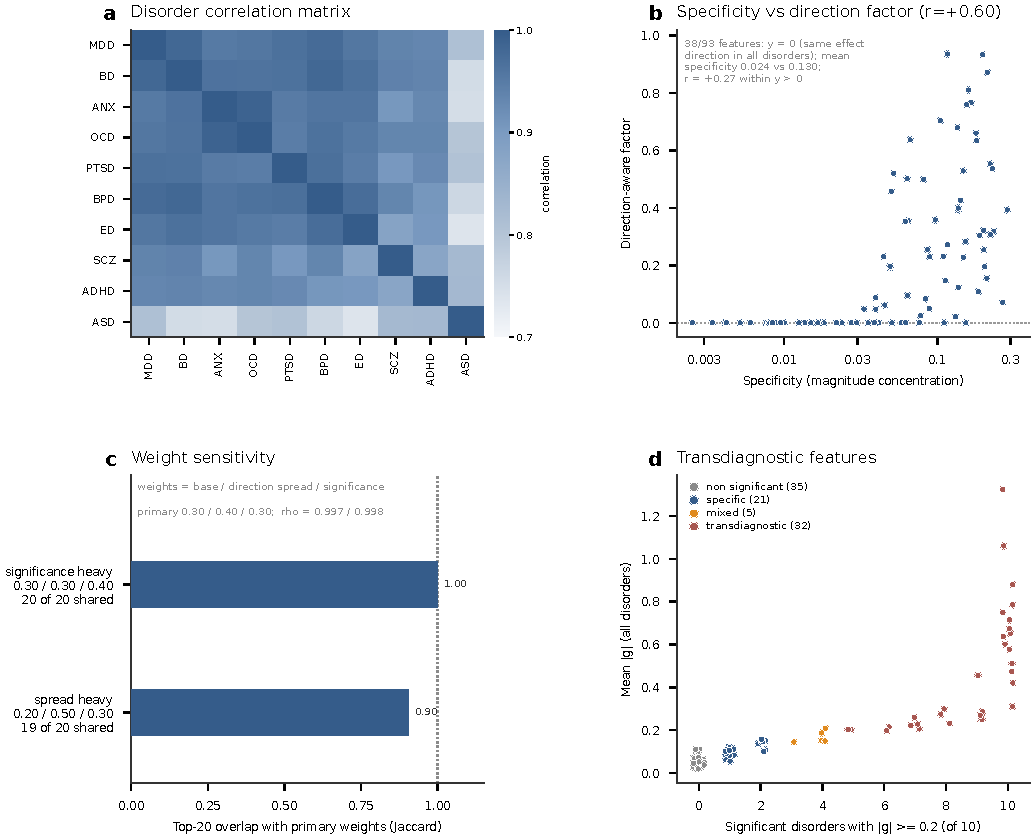
\includegraphics[width=0.98\linewidth]{figures/si2_feature_detail_lyc.pdf}
\caption{\textbf{Feature-level detail.} \textbf{a}, Disorder correlation matrix. \textbf{b},
Magnitude concentration (specificity) against the direction-aware factor (ratio of differential
specificity to specificity). \textbf{c}, Clinical-utility weight sensitivity: top-20 overlap
(Jaccard) between the primary weighting and two alternative weightings. \textbf{d},
Transdiagnostic features: mean $|g|$ over all disorders against the number of disorders in which
the effect is both significant and non-trivial ($|g|\ge0.2$), coloured by feature category.}
\label{fig:s2}
\end{figure}

\begin{figure}[h]\centering
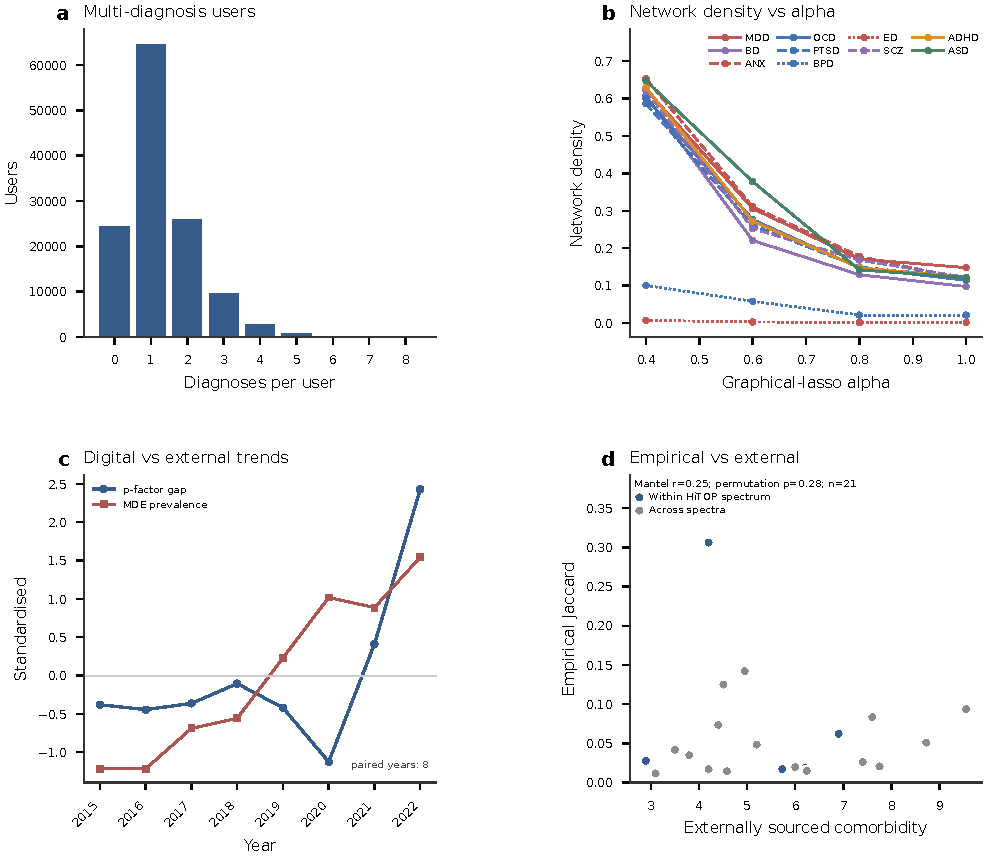
\includegraphics[width=0.98\linewidth]{figures/si3_auxiliary_validation_lyc.pdf}
\caption{\textbf{Auxiliary validation detail.} \textbf{a}, Number of diagnoses per user in the
matched cohort. \textbf{b}, Network density against the graphical-lasso penalty (colour, HiTOP
spectrum; line styles separate the disorders that share a colour). \textbf{c}, Standardised
digital p-factor gap against externally sourced epidemiology (major-depressive-episode
prevalence; 8 paired years). \textbf{d}, Empirical (cohort-overlap) comorbidity against the
externally sourced comorbidity matrix, coloured by within- versus cross-spectrum membership;
this same-cohort comparison reflects internal consistency rather than external convergence.
Mantel $r$, permutation $P$ and number of pairs given in the legend.}
\label{fig:s3}
\end{figure}

\section*{Supplementary References}
\addcontentsline{toc}{section}{Supplementary References}
\noindent External comorbidity sources used for the primary Mantel test (Supplementary Table~4).
\begin{enumerate}
\item Hasin DS, Sarvet AL, Meyers JL \emph{et al.} Epidemiology of adult \emph{DSM-5} major depressive disorder and its specifiers in the United States. \emph{JAMA Psychiatry} \textbf{75}, 336--346 (2018). \href{https://doi.org/10.1001/jamapsychiatry.2017.4602}{doi:10.1001/jamapsychiatry.2017.4602}
\item Ruscio AM, Stein DJ, Chiu WT, Kessler RC. The epidemiology of obsessive--compulsive disorder in the National Comorbidity Survey Replication. \emph{Mol. Psychiatry} \textbf{15}, 53--63 (2010). \href{https://doi.org/10.1038/mp.2008.94}{doi:10.1038/mp.2008.94}
\item Udo T, Grilo CM. Psychiatric and medical correlates of \emph{DSM-5} eating disorders in a nationally representative sample of adults in the United States. \emph{Int. J. Eat. Disord.} \textbf{52}, 42--50 (2019). \href{https://doi.org/10.1002/eat.23004}{doi:10.1002/eat.23004}
\item Hartman CA, Larsson H, Vos M \emph{et al.} Anxiety, mood and substance use disorders in adult men and women with and without attention-deficit/hyperactivity disorder: a substantive and methodological overview. \emph{Neurosci. Biobehav. Rev.} \textbf{151}, 105209 (2023). \href{https://doi.org/10.1016/j.neubiorev.2023.105209}{doi:10.1016/j.neubiorev.2023.105209}
\item Kessler RC, Birnbaum H, Demler O \emph{et al.} The prevalence and correlates of nonaffective psychosis in the National Comorbidity Survey Replication (NCS-R). \emph{Biol. Psychiatry} \textbf{58}, 668--676 (2005). \href{https://doi.org/10.1016/j.biopsych.2005.04.034}{doi:10.1016/j.biopsych.2005.04.034}
\item Smith SM, Goldstein RB, Grant BF. The association between post-traumatic stress disorder and lifetime \emph{DSM-5} psychiatric disorders among veterans: data from the National Epidemiologic Survey on Alcohol and Related Conditions-III (NESARC-III). \emph{J. Psychiatr. Res.} \textbf{82}, 16--22 (2016). \href{https://doi.org/10.1016/j.jpsychires.2016.06.022}{doi:10.1016/j.jpsychires.2016.06.022}
\item Hudson JI, Hiripi E, Pope HG, Kessler RC. The prevalence and correlates of eating disorders in the National Comorbidity Survey Replication. \emph{Biol. Psychiatry} \textbf{61}, 348--358 (2007). \href{https://doi.org/10.1016/j.biopsych.2006.03.040}{doi:10.1016/j.biopsych.2006.03.040}
\end{enumerate}

\end{document}